\chapter{Introducción}
	
	Este capítulo del documento se propone a describir, en leves pinceladas, los objetivos principales que el proyecto debe de completar.
	
		\section{Introducción}
	
	
			En los últimos años, el volumen de datos que una empresa o entidad necesita y/o es capaz de gestionar o manipular, ha aumentado de forma vertiginosa. Además del volumen de datos a manipular, nos damos cuenta de que para acceder a lo diversos datos es necesario muchas veces establecer comunicaciones con los diversos recursos existentes para alcanzar el objetivo.
			
			\vspace{5mm}
			
			
			 Con el objeto de facilitar este proceso de recuperación de información almecenada en sistemas y fuentes de datos hetereogéneas, dentro de la empresa	CIC, se está desarrollando una aplicación denominada LUCA. Para	facilitar este proceso de recuperación de información, LUCA proporciona un lenguaje común para todas las fuentes de datos a unificar, permitiendo al
			usuario abstraerse de los detalles de cada fuente.
			
			\vspace{5mm}
			
			 Actualmente LUCA proporciona mecanismos o abstracciones para permitir al	usuario recuperar de manera uniforme información de diferentes fuentes de datos. No obstante, LUCA actualmente sólo es capaz recuperar información de una única fuente de datos a la vez. Por tanto, cuando es necesario combinar información procedente de distintas fuentes, el propio usuario es el que debe realizar dicho	proceso de composición, ejecutando cada consulta a mano, y utilizando las salidas de cada una de ellas como las entradas de las siguientes.
			 
			 \vspace{5mm}
			 
			 El objetivo de este proyecto es facilitar dicho proceso de composición al usuario mediante el desarrollo de un mecanismo gráfico para la especificación de estos procesos de composición de consultas.
			 
	 
	 	\section{Planificación del proyecto}
	 	
	 	En este apartado se describe la metodología de desarrollo que ha sido utilizada para la cumplimentación del proyecto. 
	 	
	 	\vspace{5mm}
	 	
	 	
	 	En el proyecto se optó por utilizar una metodología en cascada, en la que de forma iterativa se va puliendo el producto hasta completar los requisitos y objetivos establecidos.
	 	
	 	\vspace{5mm}
	 	
	 	\begin{figure}[h]
	 		\centering
	 		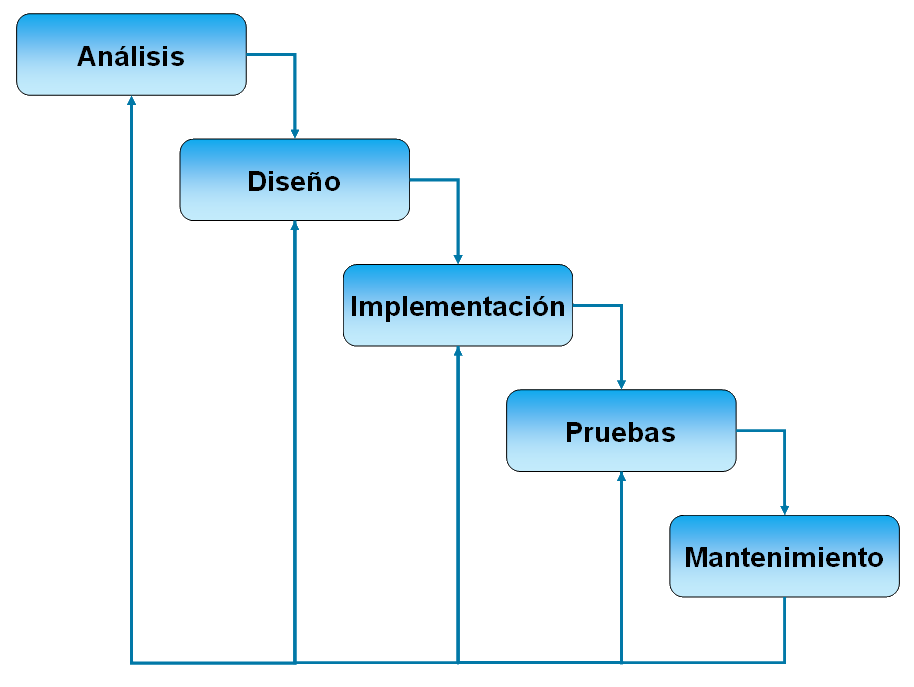
\includegraphics[scale=0.5]{modelo-en-cascada.png}
	 		\caption{Metodología En Cascada}\label{fig:modelo-en-cascada}
	 	\end{figure}
 	
 		\vspace{5mm}
 	
 		Acorde a la imagen mostrada previamente, la primera etapa de la metodología que se llevo a cabo para la cumplimentación del proyecto fue el análisis de los requisitos y objetivos del proyecto. El objetivo de esta etapa es describir de forma detallada el conjunto del requisitos y funcionalidades necesarias para la satisfacción del stakeholder y la completitud del sistema.
 		
 		\vspace{5mm}
 		
 		Una vez en posesión de la especificación de requisitos, el siguiente paso fue definir el diseño arquitectónico del proyecto en bloques independientes que puediesen ser elaborados y probados de forma aislada. Otro requisito importante que se tuvo que tener en cuenta fue, que el producto debe de estar diseñado para poder hacer frente a futuros incrementos.
 		
 		\vspace{5mm}
 		
 		Utilizando el diseño arquitectónico ya definido, se focalizó el esfuerzo en el diseño de la aplicación. En esta se tuvo en cuenta que se pretenden realizar dos elaboraciones o componentes software:
 		
 		\vspace{5mm}
 		
 		\begin{itemize}
 			\item En una primera instancia se desarrollara un componente genérico cuya funcionalidad es de índole gráfica, por lo que no precisa de una desarrollo en capas común, ya que consta unicamente de un modelo de datos y una implementación web a través del Framework GO.JS, así la integración con Vaadin\cite{vaadin}.
 			
 			\item En una segunda instancia se desarrollará una aplicación incremento del producto actual ya elaborado llamado LUCA. El cuál sigue un patrón MVP \cite{mvp}, y esta elaborado en Spring\cite{spring}.
 		\end{itemize}
 	
 		\vspace{5mm}
 		
 		Para aplicación desarrollado con Spring, se creó una base de datos relacional asociada, la cuál servirá de fuente de persistencia de los datos almacenados.
 		
 		\vspace{5mm}
 		
 		Tras la especificación de la base de datos comenzó un proceso iterativo de implementación, verificación y pruebas en el que en función de los diversos requisitos se fue completando el proyecto.
 		 
	 
	 
		\section{Estructura del documento}
		
		Esta sección se propone describir la ingeniería de requisitos llevada a cabo, así como, profundizar en el diseño arquitectónico. También como introducción inicial, se relatará de forma breve y concisa la librería javascript GO.JS y el framework Vaadin.
		
		\vspace{5mm}
		
		 En primera instancia explicará el proceso de captura y especificación de requisitos llevado a cabo, así como, la toma de decisiones seguidas. También se centrará en detallar y explicar las decisiones para la especificación de la base de datos, que deberán de estar de acuerdo con las implementación actuales de las bases de datos de LUCA, y con la especificacion basada en Spring.	Por último se explicará el proceso de desarrollo de las capas de repositorio, servicios y presentación.
		
		

	 